\documentclass[12pt]{article}

\usepackage{graphicx, subcaption}
\usepackage[margin = 1in]{geometry}
\usepackage[font={footnotesize}]{caption}
\usepackage{indentfirst}
\usepackage{color}
\usepackage{float}
\usepackage{url}



\begin{document}
\title{Will's Latex Homework}
\author{I guess this is required so my name is Will Schultz}
\date{\today Yeah its kinda late}

\maketitle

\section{PART 1}
\subsection{Bullets}

I enjoyed:

\begin{itemize}
	\item I enjoyed helping Armando understand what was going on
	\item I enjoyed being high as fuck presenting my final project... (Actually I didn't really like that too much but it was chill)
\end{itemize}

\subsection{Numbering}

What I disliked:

\begin{enumerate}
	\item I disliked how Charman's problem sets got in the way of me spending too much time on this class
	\item I also disliked .... idk Im sure there was something else 
\end{enumerate}

\section{PART 2}

Time to write an equation...

\begin{equation}
	\sum_{j=0}^{n}(-1)^j\partial_{\mu_1 \ldots \mu_j}^j\left(\frac{\partial L}{\partial f_{i,\mu_1 \ldots \mu_j}}\right) = 0
\end{equation}

Idk what the $\mu_1 \ldots \mu_j$ means but Im sure if I took a break from problem sets I would find it.

\section{PART 3}

Here is the table you requested:

\begin{table}[H]
  \centering
  \begin{tabular}{|l|c|r|}
    \hline
     Favorite Foods & Favorite Bands & Favorite IDL Commands \\
      \hline
   Pizza & Led Zeppelin & display \\
   Cheese Fries & The Who & mrdfits()  \\
   My Dad's Chili & Rolling Stones & where()  \\ \hline

 \end{tabular}
  \caption{If I was more creative I would add more about these, but I think all that is warranted is the Led Zepplin is the best followed closely by the Who.}
  \label{tab:favs}
\end{table}

Why do we not have to use references with the table like this: See Table \ref{tab:favs} for the best bands ever.

\section{PART 4}

I don't know what the .ps files are .... but I thought you would enjoy this.

\begin{figure}[H]
	\centering
        	
\includegraphics[width = \linewidth]{What_I_Learned.jpg}
        	\caption{Hey, at least it is a .ps file, or I have a copy of this as a .ps which I tried to put into the include graphics but it didn't work and because of Charman's problem set, I will just use the jpeg. I apologize for the lack of .ps, but hey ... "Check it out!"}
        \label{fig:the1nonly} 
\end{figure}

\section{PART 5}

\begin{figure}[H]
  \centering
    \begin{minipage}[t]{.45\textwidth}
      \centering
        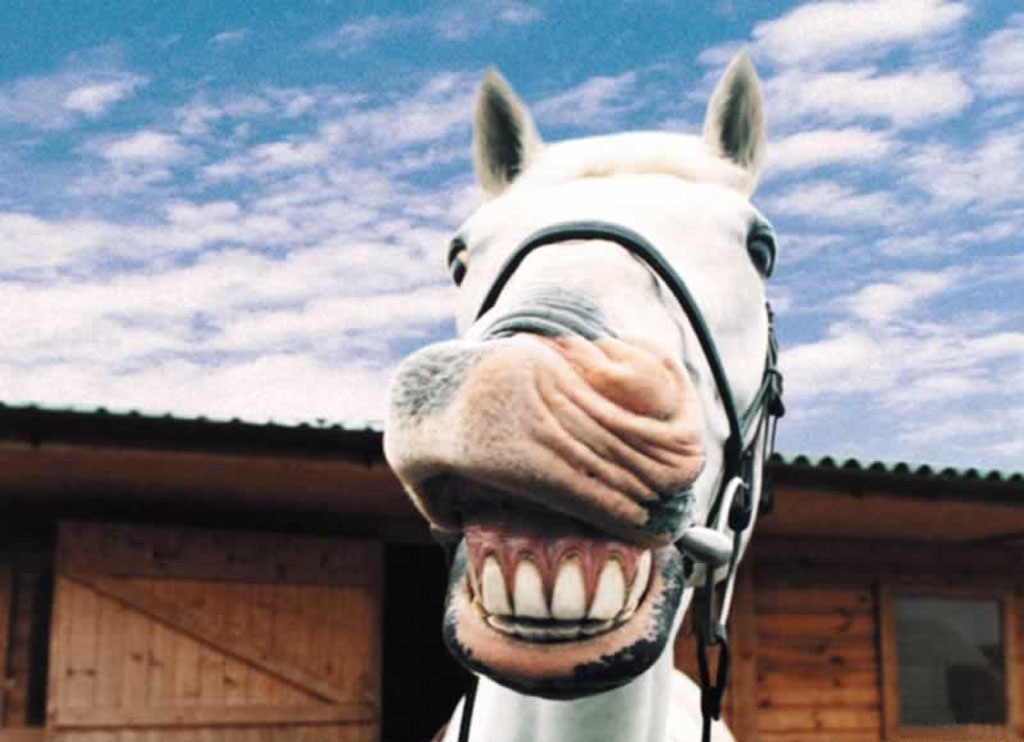
\includegraphics[width = \linewidth]{funny-horse.jpg}  
        \caption{LOL. Horse.}
    \label{fig:horse}
    \end{minipage}
    \quad
    \begin{minipage}[t]{.45\textwidth}
      \centering
        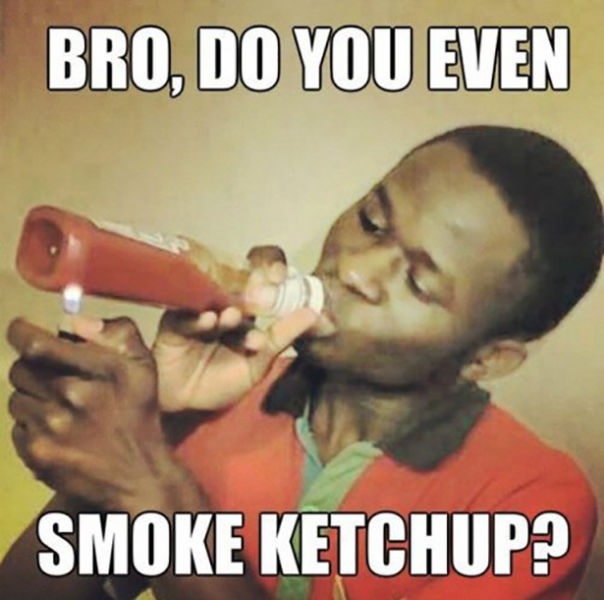
\includegraphics[width = \linewidth]{ketchup.jpg}
        \caption{Who doesn't these days?}
        \label{fig:ketchup}
    \end{minipage}
\end{figure}

\end{document}
